\chapter{Implementación}

\section{Propuesta considerada}

Examinando las técnicas anteriormente revisadas, se llega al punto de que lo más factible es trabajar con las cadenas de secuencias utilizando un arreglo que las encadene una a una. Recordando los objetivos que se tienen para esta memoria, estas son:

\begin{enumerate}
\item Obtener la cantidad total de diferentes residuos de aminoácidos de tamaño $k =$ 1 hasta 50 que existen para las bases de datos de UniProt-SwissProt y UniProt-TrEMBL.
\item Encontrar para cada caso anterior cuáles son los residuos de aminoácidos que más se repiten.
\end{enumerate}

Para realizar la primera tarea, será necesario construir un \textit{suffix array} el cual será la base del arreglo LCP para realizar este objetivo. Considerando un ejemplo sencillo como la palabra BANANA\$:

\begin{table}[H]
	\centering
	\begin{tabular}{c l}
		\textit{\textbf{SA[]}} & \textit{\textbf{sufijo}}\\
		6 & \$\\
		5 & A\$\\
		3 & ANA\$\\
		1 & ANANA\$\\
		0 & BANANA\$\\
		4 & NA\$\\
		2 & NANA\$\\
	\end{tabular}
\end{table}

Se puede apreciar que los números asociados a cada sufijo ya están ordenados como si fuera un arreglo de sufijos. Es posible obtener la cantidad total de diferentes substrings que componen esta palabra utilizando el arreglo LCP de la siguiente forma. Introduciendo los 2 siguientes conceptos:

{\it{length}}('X') = Largo de caracteres de la palabra 'X'.\\
{\it{LCP}}('Y','Z') = Prefijo más largo en común ({\it{Longest Common Prefix}}) entre los substrings 'Y' y 'Z'.

Y partiendo según el orden alfabético dado anteriormente, se hace el siguiente ejercicio:

Largo primer sufijo ordenado ('\$') = 1 = $var$\\
Comienzo de pares de sufijos:
\begin{enumerate}
	\item ('\$','A\$'): $var +=$ {\it{length}}('\$A') - {\it{LCP}}('\$','\$A')\\
	$var=var+2-0 =>  1+2=3$

	\item ('A\$','ANA\$'): $var +=$ {\it{length}}('ANA\$') - {\it{LCP}}('A\$','ANA\$')\\
	$var=var+4-1 =>  3+3=6$
	
	\item ('ANA\$','ANANA\$'): $var +=$ {\it{length}}('ANANA\$') - {\it{LCP}}('ANA\$','ANANA\$')\\
	$var=var+6-3 =>  6+3=9$
	
	\item ('ANANA\$','BANANA\$'): $var +=$ {\it{length}}('BANANA\$') - {\it{LCP}}('ANANA\$','BANANA\$')\\
	$var=var+7-0 =>  9+7=16$
	
	\item ('BANANA\$','NA\$'): $var +=$ {\it{length}}('NA\$') - {\it{LCP}}('BANANA\$','NA\$')\\
	$var=var+3-0 =>  16+3=19$
	
	\item ('NA\$','NANA\$'): $var +=$ {\it{length}}('NANA\$') - {\it{LCP}}('NA\$','NANA\$')\\
	$var=var+5-2 =>  19+3=22$
	
\end{enumerate}

Cantidad de diferentes substrings que hay en BANANA\$: 22.

Lo que se hace en este caso es crear una variable y guardar la longitud del primer sufijo del SA (en este caso \$) para luego realizar una comparación entre los sufijos consecutivos $i$ y $j$ adicionando en cada caso a la variable las longitudes respectivas de los sufijos $j$, y además \textbf{se le resta el prefijo común más largo entre estos sufijos consecutivos}:

\begin{table}[H]
	\centering
	\label{propuesta-1}
	\begin{tabular}{c c l}
		\textit{\textbf{SA[]}} & \textit{\textbf{LCP[]}} &\textit{\textbf{sufijo}}\\
		6 & 0 & \$\\
		5 & 0 & A\$\\
		3 & 1 & ANA\$\\
		1 & 3 & ANANA\$\\
		0 & 0 & BANANA\$\\
		4 & 0 & NA\$\\
		2 & 2 & NANA\$\\
	\end{tabular}
\caption{SA y arreglo LCP de la palabra BANANA\$}
\end{table}

Entonces, particularizando el problema, ¿cómo sería posible obtener la cantidad total de diferentes substrings de un determinado tamaño? La clave está en el \textbf{arreglo LCP} obtenido, el cual se puede utilizar desde 2 perspectivas para realizar esta tarea.

\subsection{Restando la cantidad máxima posible de diferentes substrings}

Primero que todo hay que considerar la cantidad potencial máxima de diferentes substrings de tamaño $k$ que se pueden obtener (la fórmula es $n-k+1$ donde $n$ es el largo de la palabra) y luego se recorre el arreglo LCP utilizando el valor de $k$ como un comparador.
Por ejemplo, de la palabra BANANA\$ a simple vista se sabe que los diferentes substrings de tamaño 1 que se encuentran son 4, que son A, B, N y \$. Usando la fórmula mencionada en el párrafo anterior se tiene que $7-1+1=7$ es la cantidad máxima de substrings de tamaño 1 de esta palabra. Recorriendo el arreglo LCP es necesario encontrar aquellos valores que sean \textbf{mayores o iguales que $k$} para restarlos a la cantidad máxima de diferentes substrings, porque ese valor indica en el arreglo de sufijos si determinado sufijo se \textbf{repite más de una vez}, por consiguiente esto indica que disminuye en una unidad la cantidad total de diferentes substrings de determinado tamaño. Aplicando en el caso anterior:

Máxima cantidad de diferentes substrings de tamaño 1 para BANANA\$: $DS = 7$

$a)$ $LCP[0]=0 =>$ DS se mantiene $=> DS=7$\\
$b)$ $LCP[1]=0 =>$ DS se mantiene $=> DS=7$\\ 
$c)$ $LCP[2]=1 =>$ $DS=7-1=6$\\ 
$d)$ $LCP[3]=3 =>$ $DS=6-1=5$\\
$e)$ $LCP[4]=0 =>$ DS se mantiene $=> DS=5$\\
$f)$ $LCP[5]=0 =>$ DS se mantiene $=> DS=5$\\
$g)$ $LCP[6]=2 =>$ $DS=5-1=4$ 

Diferentes substrings en total de tamaño 1 en la palabra BANANA\$: 4.

Para los tamaños 2 hasta 7 (palabra completa) los diferentes substrings encontrados son los siguientes:\\

\begin{table}[H]
\centering
\label{propuesta-12}
\begin{tabular}{|c|c|c|}
\hline
Tamaño 2     & Tamaño 3      &  Tamaño 4   \\
Substrings totales: 6      &  Substrings totales: 5    & Substrings totales: 4   \\
Elementos LCP $\geq$ 2: 2       & Elementos LCP $\geq$ 3: 1       & Elementos LCP $\geq$ 4: 0      \\
DS de tamaño 2: $6-2 = 4$      & DS de tamaño 3: $5-1 = 4$          & DS de tamaño 4: $4-0 = 4$            \\ \hline
Tamaño 5     & Tamaño 6      &  Tamaño 7   \\
Substrings totales: 3      &  Substrings totales: 2    & Substrings totales: 1   \\
Elementos LCP $\geq$ 5: 0       & Elementos LCP $\geq$ 6: 0       & Elementos LCP $\geq$ 7: 0      \\
DS de tamaño 5: $3-0 = 3$      & DS de tamaño 6: $2-0 = 2$          & DS de tamaño 7: $1-0 = 1$            \\ \hline
\end{tabular}
\end{table}

Sumando los DS encontrados entre los tamaños 1 hasta 7 el valor es de $4+4+4+4+3+2+1=22$, obteniendo el mismo valor de antes.

\subsection{Aumentando la cantidad de diferentes substrings desde 0 considerando determinados tamaños de LCPs consecutivos}

Esta segunda perspectiva considera recorrer el arreglo LCP con una pequeña variación, la que sería mover el primer elemento del arreglo (que siempre será 0) y dejarlo en la última posición desde izquierda a derecha:

\begin{table}[h]
\centering
\label{propuesta-2}
\begin{tabular}{|l|l|l|l|l|l|l|l|l|l|l|l|l|l|l|}
\cline{1-7} \cline{9-15}
0 & 0 & 1 & 3 & 0 & 0 & 2 & -\textgreater & 0 & 1 & 3 & 0 & 0 & 2 & 0 \\ \cline{1-7} \cline{9-15} 
\end{tabular}
\caption{Arreglo LCP (tabla izquierda) mueve su primer elemento (0) hacia la última posición (tabla derecha).}
\end{table}

El motivo de esto es identificar el prefijo común más largo entre los 2 sufijos consecutivos entre los sufijos $x$ e $y$ considerando al {\textbf{primero o sufijo \textit{x}}} como el sufijo de referencia:

\begin{table}[H]
	\centering
	\label{propuesta-21}
	\begin{tabular}{c c l}
		\textit{\textbf{SA[]}} & \textit{\textbf{LCP[]}} &\textit{\textbf{sufijo}}\\
		6 & 0 & \$\\
		5 & 1 & A\$\\
		3 & 3 & ANA\$\\
		1 & 0 & ANANA\$\\
		0 & 0 & BANANA\$\\
		4 & 2 & NA\$\\
		2 & 0 & NANA\$\\
	\end{tabular}
\caption{SA y arreglo LCP modificado de la palabra BANANA\$}
\end{table}

Para que sea más entendible, el último valor del arreglo LCP modificado es 0 ya que NANA\$ es el último sufijo, y no tiene un sufijo posterior con el cual compararse.

En esta ocasión no se considerará la máxima cantidad de diferentes substrings de tamaño $k$ ($n-k+1$) ya que todo se obtendrá del \textit{suffix array} y de su arreglo LCP correspondiente, y el realizar esta modificación en el arreglo LCP permitirá lograr el segundo objetivo para este trabajo, que es el de encontrar a los conjuntos de péptidos que más se repiten para un determinado tamaño. Se puede ejemplificar esto con la búsqueda de los diferentes substrings de tamaño 3 en la palabra BANANA\$:

Se inicializa con $DS = 0$.

a) $LCP[0]=0 =>$ se mantiene $=> DS=0$ ya que el tamaño del sufijo es menor a 3 ($SA[0]=$ \$).\\
b) $LCP[1]=1 =>$ se mantiene $=> DS=0$ ya que ocurre el mismo fenómeno de antes ($SA[1]=$ A\$).\\ 
c) $LCP[2]=3 => SA[2] =$ ANA\$, este sufijo con su siguiente sufijo consecutivo tiene como \textit{longest common prefix} a ANA, por lo tanto se sabe que ANA se repite al menos 2 veces en la palabra; por ahora se seguirá dejando $DS = 0$.

Aquí viene la premisa del LCP consecutivo, ya que si el siguiente valor del arreglo LCP (para este caso $LCP[3]$) fuera mayor o igual que 3, entonces se tendría una nueva repetición del prefijo ANA, por lo tanto ahora serían 3 las veces que este prefijo estaría repetido en la palabra. Entendiéndolo de manera más formal, se tendrían \textbf{$l$ valores consecutivos desde la posición $s$ del arreglo LCP que serían mayores que $k$ (que para este caso es 3)}, entregando un total de $l+1$ repeticiones del sufijo $SA[s]$ de tamaño $k$. En caso contrario (valor del arreglo LCP menor que 3), se acabarían las repeticiones de determinado sufijo y se agrega una unidad al total de diferentes substrings encontrados.

d) $LCP[3]=0 =>$ Aquí el valor es menor que 3, por lo tanto $DS=0+1=1$ y se tiene que ``ANA'' se repite 2 veces.\\
e) $LCP[4]=0 =>$ Tamaño $SA[4] = 7$, $SA[4,3] =$ BAN, por lo tanto $DS=1+1=2$.\\
f) $LCP[5]=2 =>$ Tamaño $SA[5] = 3$, $SA[5,3] =$ NA\$, por lo tanto $DS=2+1=3$.\\
g) $LCP[6]=0 =>$ Tamaño $SA[6] = 5$, $SA[6,3] =$ NAN, por lo tanto $DS=3+1=4$.\\

Por consiguiente, se tiene que los diferentes substrings de tamaño 3 para la palabra BANANA\$ son 4, ANA que se repite 2 veces, BAN, NA\$ y NAN, que se repiten solo una vez. Sumando estas cantidades se tiene un valor de 5, que es el \textbf{número total de substrings de tamaño 3} ($n-k+1$).

Por ende para la realización del algoritmo se utilizará esta segunda premisa, considerando las restricciones pertinentes para este trabajo.

\subsection{Restricciones para la propuesta}

Primero que todo, se extraerán las secuencias de polipéptidos de los archivos .fasta y se alinearán en una \textbf{única gran cadena} donde cada secuencia estará unida por un signo \$, con esto será posible identificar en los arreglos si cierto sufijo está compuesto por este signo o no, de esa forma descartarlo dentro de los diferentes residuos de aminoácidos que se cuentan:

\begin{table}[h]
\centering
\label{propuesta-22}
\begin{tabular}{c}
$\ldots$MPSTLQVLAKKVLKENDHISR\$EYHILKCWHEAPIILCFNGSKQM$\ldots$\\ 
\end{tabular}
\caption{2 secuencias enlazadas en una cadena general utilizando el signo \$ como unión.}
\end{table}

Para esta cadena grande (de largo $m$), el arreglo de sufijos y el arreglo LCP tendrán tamaño $m$, por lo cual para determinar los diferentes substrings de tamaño $k$ y aquellos substrings que más se repiten se debe recorrer el arreglo LCP completo, considerando:

\begin{enumerate}
\item Si el largo del sufijo es mayor o igual a $k$, entonces el arreglo LCP puede ser analizado, en caso contrario se omite y se continúa al siguiente valor del arreglo LCP.
\item Si el prefijo del sufijo revisado \textbf{solamente esté compuesto por los 20 aminoácidos conocidos} \cite{biomolecula}. Otros aminoácidos que no han sido definidos, como B, J, O, U o X serán omitidos para este problema (si son parte del substring del sufijo revisado, se omitirá y se continuará al arreglo LCP siguiente) y considerados como prohibidos \cite{aminoacids}. El signo \$ también será incluído a este grupo de carácteres prohibidos.
\end{enumerate}

Con respecto a esto es posible obtener los substrings diferentes y la cantidad de repeticiones que posee cada uno de estos, para posteriormente guardarlos en algun tipo de lista o vector. El problema es tratar de acceder a aquellos substrings que más se repiten, detalle que se verá en la siguiente sección.

\section{Algoritmo desarrollado}

Para la obtención de los diferentes substrings se realizó un código implementado en lenguaje C++ siguiendo varios puntos, en primera instancia para la base de datos de SwissProt y TrEMBL se realizó una extracción previa de datos.

El archivo ``uniprot\_sprot.fasta'' está compuesto por 555426 proteínas con un peso total de 268 MB, mientras que el ``uniprot\_trembl.fasta'' está compuesto por 88032926 proteínas con un peso de 40 GB. Para ambos archivos la construcción del arreglo de sufijos y el arreglo LCP serán diferentes pero recibirán la misma cadena enlazada, cuya construcción será explicada en la siguiente sección.

\subsection{Extracción de proteínas desde el archivo .fasta}

EL archivo \textit{.fasta} entrega cada polipéptido con un código o ID (que comienza con un $>$), a continuación en la misma línea se tiene al nombre taxativo de la proteína, y en la línea siguiente viene la cadena como tal, para luego repetir el proceso:

\begin{figure}[h]
    \centering
    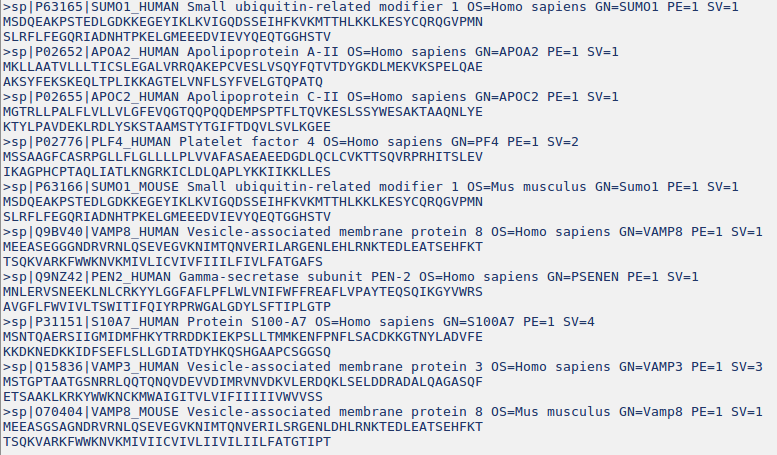
\includegraphics[width=0.9\textwidth]{./images/fastadefecto.png}
    \caption{Archivo \textbf{.fasta} por defecto con varias proteínas}
    \label{fig:image5}
\end{figure}

Para extraer las cadenas se implementó el siguiente código en C++:

\begin{lstlisting}[language=C++, caption=Creación de cadena de proteínas]
ifstream fin("uniprot_sprot.fasta"); //abrir archivo base
if(!fin){
	cerr << "Couldn't open the input file!";
	return(1);
}
ofstream outputfile; //crear archivo destino de cadena
outputfile.open("substrings.txt"); //definir nombre de archivo a crear
string line; 
int cantidad_ss = 1;

getline(fin, line); 
getline(fin, line); //tomar secuencia (1)

while(fin){
	if(line[0] == '>'){ // revisar primer elemento del string (2)
		outputfile << "$";
		cantidad_ss = cantidad_ss + 1;
	}
	else{
		outputfile << line;
	}
getline(fin, line); // continuar con la siguiente linea (3)
}

outputfile.close();
\end{lstlisting}

Lo que hace este código es crear un nuevo archivo ``substrings.txt'' en la variable \textbf{outputfile} donde se guardará la cadena de proteínas. Con \textit{getline} se lee la primera ĺinea del archivo .fasta que está guardada en la variable \textbf{fin}, e inmediatamente después se llama nuevamente a \textit{getline} para leer la segunda línea del archivo .fasta, que es \textbf{una secuencia o parte de ella} (1). Luego se condiciona a realizar una de las 2 tareas siempre y cuando el archivo .fasta no se haya leído completamente: 

\begin{enumerate}
\item Si el primer elemento de la línea leída del archivo .fasta es $>$, significa que se llegó al final de una secuencia, por lo tanto es el comienzo de la siguiente (es la linea de definición de la proteína), en ese caso se le agrega el signo \$ al archivo destino como separador (2). 
\item En caso contrario, se le agrega directamente la línea completa al archivo destino, ya que esta línea solamente está compuesta por \textbf{la secuencia en sí}.
\end{enumerate}

Finalmente se vuelve a llamar a \textit{getline} para continuar con la siguiente línea del archivo .fasta (3).

En resumen el formato del nuevo archivo ``substrings.txt'' es una sola línea que tiene concatenada todas las proteínas:

\begin{table}[h]
\centering
\label{propuesta-23}
\begin{tabular}{c}
TSCPGGNHPVCCSTDLCNK\$MKTL$\ldots$SDLT\$LKCNKLVPLFYKTCP\\ 
\end{tabular}
\caption{Ejemplo de cadena encontrada en el archivo destino}
\end{table}

Teniendo esta gran línea ya se puede construir el arreglo de sufijos y el arreglo LCP. Considerar como dato relevante que guardando esta cadena en una variable tipo \textit{string} cada caracter ocupa el tamaño de 1 byte de capacidad \cite{manipulatingstrings}, y esto determinará de qué manera se construirán los arreglos para la solución de este problema.

Por defecto se tiene que el tamaño de UniProt-SwissProt es de 268 MB y su cadena de proteínas tiene un peso de 199 MB, mientras que para UniProt-TrEMBL su tamaño por defecto es de 40 GB y su cadena de proteínas posee un peso de 30 GB, si se tiene en consideración que para guardar la cadena en una variable esta se almacena en la memoria RAM del ordenador. En primera instancia no hay problema con la base de datos de SwissProt ya que el espacio ocupado es suficiente si se trabaja en un computador normal (si se guardan los arreglos en una variable tipo \textit{vector}, cada elemento del vector pesa 4 bytes), pero para la cadena creada en función de UniProt-TrEMBL parece ser más complejo, ya que el string para almacenar la cadena requeriría 30 GB de memoria RAM, inclusive ocupando un servidor con 50 GB de capacidad de RAM sería inviable construir los arreglos (en cálculos sencillos se necesitaría de una RAM de al menos 300 GB para realizar esta tarea). Una posible solución para esto se revisará más adelante en la implementación para la base de datos UniProt-TrEMBL.

\subsection{Implementación solución para base de datos UniProt-SwissProt}

Para la implementación del algoritmo se trabajó en base al algoritmo de Kasai (poner cite) para obtener el arreglo LCP en base al arreglo de sufijos.

\subsubsection{Arreglo de sufijos}
